\documentclass{standalone}
\usepackage{tikz}
\usetikzlibrary{patterns, positioning}
\usepackage[sfdefault]{ClearSans} %% option 'sfdefault' activates Clear Sans as the default text font
\usepackage[T1]{fontenc}

\begin{document}
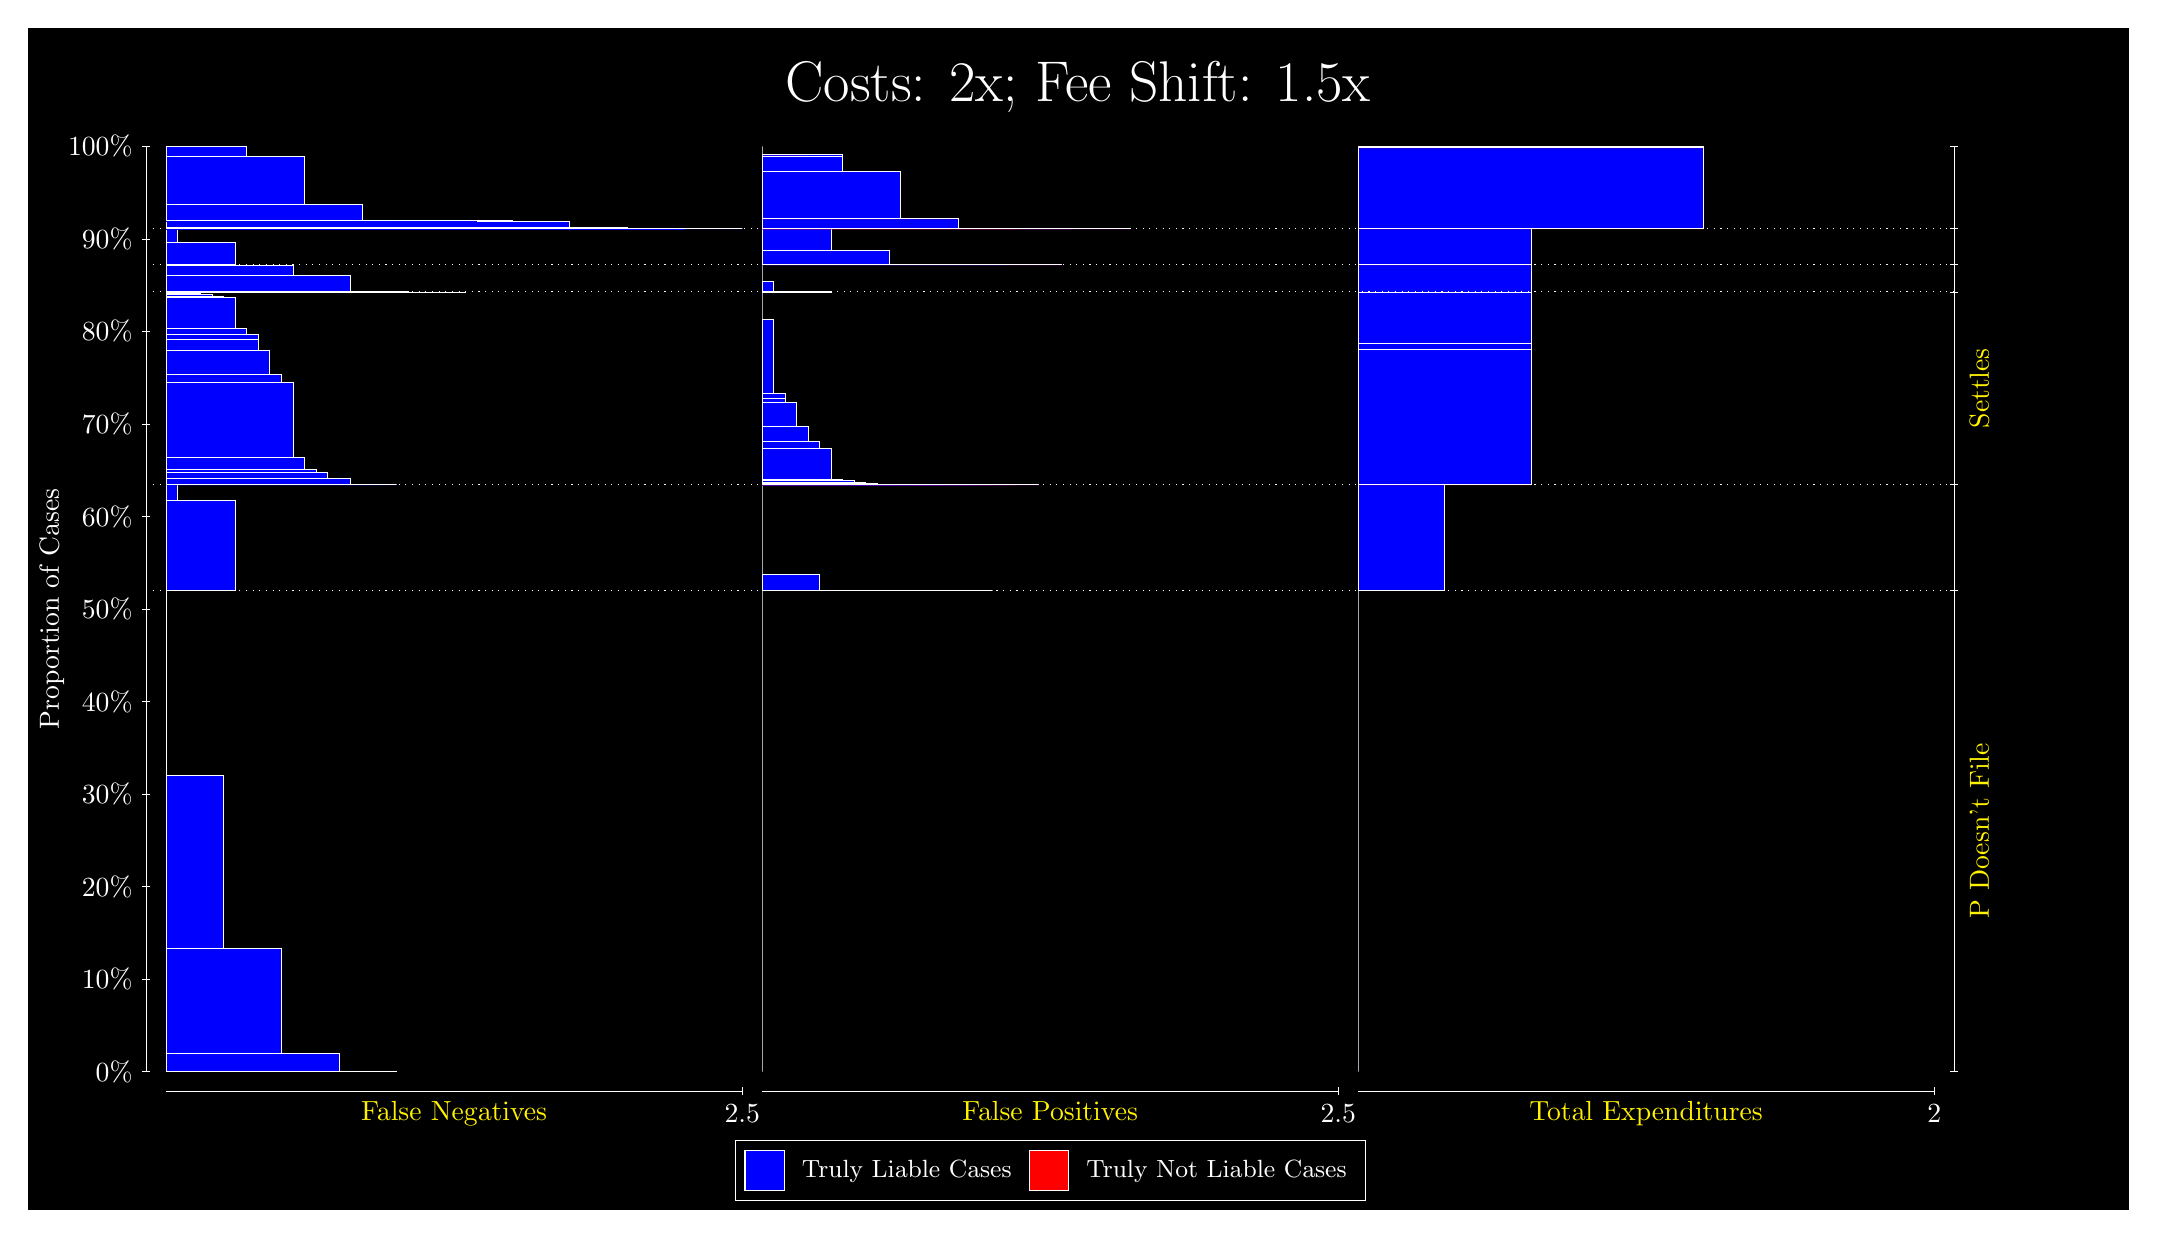
\begin{tikzpicture}
\draw[fill=black] (0,0) rectangle (26.667,15);
\draw[text=white] (0,13.5) rectangle (26.667,15) node[midway] {\huge Costs: 2x; Fee Shift: 1.5x};
\draw[white, very thin] (1.5,1.75) -- (1.5,13.5);
\node[rotate=90, text=white, anchor=center] at (0.3, 7.625) {Proportion of Cases};
\draw[white, very thin] (1.45,1.75) -- (1.55,1.75);
\node[text=white, anchor=east] at (1.45, 1.75) {0\%};
\draw[white, very thin] (1.45,2.925) -- (1.55,2.925);
\node[text=white, anchor=east] at (1.45, 2.925) {10\%};
\draw[white, very thin] (1.45,4.1) -- (1.55,4.1);
\node[text=white, anchor=east] at (1.45, 4.1) {20\%};
\draw[white, very thin] (1.45,5.275) -- (1.55,5.275);
\node[text=white, anchor=east] at (1.45, 5.275) {30\%};
\draw[white, very thin] (1.45,6.45) -- (1.55,6.45);
\node[text=white, anchor=east] at (1.45, 6.45) {40\%};
\draw[white, very thin] (1.45,7.625) -- (1.55,7.625);
\node[text=white, anchor=east] at (1.45, 7.625) {50\%};
\draw[white, very thin] (1.45,8.8) -- (1.55,8.8);
\node[text=white, anchor=east] at (1.45, 8.8) {60\%};
\draw[white, very thin] (1.45,9.975) -- (1.55,9.975);
\node[text=white, anchor=east] at (1.45, 9.975) {70\%};
\draw[white, very thin] (1.45,11.15) -- (1.55,11.15);
\node[text=white, anchor=east] at (1.45, 11.15) {80\%};
\draw[white, very thin] (1.45,12.325) -- (1.55,12.325);
\node[text=white, anchor=east] at (1.45, 12.325) {90\%};
\draw[white, very thin] (1.45,13.5) -- (1.55,13.5);
\node[text=white, anchor=east] at (1.45, 13.5) {100\%};

\draw[white, very thin] (24.457,1.75) -- (24.457,13.5);
\draw[white, very thin] (24.407,1.75) -- (24.507,1.75);
\node[anchor=west] at (24.407, 1.75) {};
\draw[white, very thin] (24.407,7.8595) -- (24.507,7.8595);
\node[anchor=west] at (24.407, 7.8595) {};
\draw[white, very thin] (24.407,9.2042) -- (24.507,9.2042);
\node[anchor=west] at (24.407, 9.2042) {};
\draw[white, very thin] (24.407,11.651) -- (24.507,11.651);
\node[anchor=west] at (24.407, 11.651) {};
\draw[white, very thin] (24.407,11.996) -- (24.507,11.996);
\node[anchor=west] at (24.407, 11.996) {};
\draw[white, very thin] (24.407,12.455) -- (24.507,12.455);
\node[anchor=west] at (24.407, 12.455) {};
\draw[white, very thin] (24.407,13.5) -- (24.507,13.5);
\node[anchor=west] at (24.407, 13.5) {};

\draw[white, very thin, fill=blue] (1.75,1.75) rectangle (4.6775,1.7523);
\draw[white, very thin, fill=blue] (1.75,1.7523) rectangle (3.9457,1.9774);
\draw[white, very thin, fill=blue] (1.75,1.9774) rectangle (3.2138,3.3124);
\draw[white, very thin, fill=blue] (1.75,3.3124) rectangle (2.4819,5.511);
\draw[white, very thin, fill=red] (1.75,5.511) rectangle (1.75,5.511);
\draw[white, very thin, fill=blue] (1.75,5.511) rectangle (1.75,7.8595);
\draw[white, very thin, fill=blue] (1.75,7.8595) rectangle (2.6283,9.0025);
\draw[white, very thin, fill=blue] (1.75,9.0025) rectangle (1.8964,9.2033);
\draw[white, very thin, fill=red] (1.75,9.2033) rectangle (1.75,9.2033);
\draw[white, very thin, fill=blue] (1.75,9.2033) rectangle (1.75,9.2042);
\draw[white, very thin, fill=blue] (1.75,9.2042) rectangle (4.6775,9.2042);
\draw[white, very thin, fill=blue] (1.75,9.2042) rectangle (4.3848,9.2043);
\draw[white, very thin, fill=blue] (1.75,9.2043) rectangle (4.092,9.2812);
\draw[white, very thin, fill=blue] (1.75,9.2812) rectangle (3.9457,9.2863);
\draw[white, very thin, fill=blue] (1.75,9.2863) rectangle (3.7993,9.3586);
\draw[white, very thin, fill=blue] (1.75,9.3586) rectangle (3.6529,9.3934);
\draw[white, very thin, fill=blue] (1.75,9.3934) rectangle (3.5065,9.5465);
\draw[white, very thin, fill=blue] (1.75,9.5465) rectangle (3.3602,10.498);
\draw[white, very thin, fill=blue] (1.75,10.498) rectangle (3.2138,10.601);
\draw[white, very thin, fill=blue] (1.75,10.601) rectangle (3.0674,10.908);
\draw[white, very thin, fill=blue] (1.75,10.908) rectangle (2.921,11.049);
\draw[white, very thin, fill=blue] (1.75,11.049) rectangle (2.921,11.107);
\draw[white, very thin, fill=blue] (1.75,11.107) rectangle (2.7746,11.185);
\draw[white, very thin, fill=blue] (1.75,11.185) rectangle (2.6283,11.589);
\draw[white, very thin, fill=blue] (1.75,11.589) rectangle (2.4819,11.597);
\draw[white, very thin, fill=blue] (1.75,11.597) rectangle (2.3355,11.626);
\draw[white, very thin, fill=blue] (1.75,11.626) rectangle (2.1891,11.632);
\draw[white, very thin, fill=blue] (1.75,11.632) rectangle (2.1891,11.639);
\draw[white, very thin, fill=blue] (1.75,11.639) rectangle (2.0428,11.642);
\draw[white, very thin, fill=blue] (1.75,11.642) rectangle (1.8964,11.651);
\draw[white, very thin, fill=red] (1.75,11.651) rectangle (1.75,11.651);
\draw[white, very thin, fill=blue] (1.75,11.651) rectangle (1.75,11.651);
\draw[white, very thin, fill=blue] (1.75,11.651) rectangle (5.5558,11.652);
\draw[white, very thin, fill=blue] (1.75,11.652) rectangle (4.8239,11.661);
\draw[white, very thin, fill=blue] (1.75,11.661) rectangle (4.092,11.865);
\draw[white, very thin, fill=blue] (1.75,11.865) rectangle (3.3602,11.995);
\draw[white, very thin, fill=blue] (1.75,11.995) rectangle (2.6283,11.996);
\draw[white, very thin, fill=red] (1.75,11.996) rectangle (1.75,11.996);
\draw[white, very thin, fill=blue] (1.75,11.996) rectangle (2.6283,12.276);
\draw[white, very thin, fill=blue] (1.75,12.276) rectangle (1.8964,12.449);
\draw[white, very thin, fill=red] (1.75,12.449) rectangle (1.75,12.449);
\draw[white, very thin, fill=blue] (1.75,12.449) rectangle (1.75,12.455);
\draw[white, very thin, fill=blue] (1.75,12.455) rectangle (9.0689,12.455);
\draw[white, very thin, fill=blue] (1.75,12.455) rectangle (8.337,12.456);
\draw[white, very thin, fill=blue] (1.75,12.456) rectangle (7.6051,12.478);
\draw[white, very thin, fill=blue] (1.75,12.478) rectangle (6.8732,12.552);
\draw[white, very thin, fill=blue] (1.75,12.552) rectangle (6.1413,12.556);
\draw[white, very thin, fill=blue] (1.75,12.556) rectangle (5.7022,12.557);
\draw[white, very thin, fill=blue] (1.75,12.557) rectangle (5.4094,12.557);
\draw[white, very thin, fill=blue] (1.75,12.557) rectangle (4.9703,12.561);
\draw[white, very thin, fill=blue] (1.75,12.561) rectangle (4.6775,12.561);
\draw[white, very thin, fill=blue] (1.75,12.561) rectangle (4.2384,12.77);
\draw[white, very thin, fill=blue] (1.75,12.77) rectangle (3.5065,13.375);
\draw[white, very thin, fill=blue] (1.75,13.375) rectangle (2.7746,13.496);
\draw[white, very thin, fill=blue] (1.75,13.496) rectangle (2.0428,13.5);
\draw[white, very thin, fill=red] (1.75,13.5) rectangle (1.75,13.5);
\draw[white, very thin, fill=blue] (1.75,13.5) rectangle (1.75,13.5);
\draw[white, very thin, fill=red] (9.3189,1.75) rectangle (9.3189,1.75);
\draw[white, very thin, fill=blue] (9.3189,1.75) rectangle (9.3189,7.8595);
\draw[white, very thin, fill=red] (9.3189,7.8595) rectangle (12.246,7.8595);
\draw[white, very thin, fill=blue] (9.3189,7.8595) rectangle (12.246,7.8595);
\draw[white, very thin, fill=blue] (9.3189,7.8595) rectangle (11.515,7.8595);
\draw[white, very thin, fill=blue] (9.3189,7.8595) rectangle (10.783,7.8604);
\draw[white, very thin, fill=blue] (9.3189,7.8604) rectangle (10.051,8.0612);
\draw[white, very thin, fill=blue] (9.3189,8.0612) rectangle (9.3189,9.2042);
\draw[white, very thin, fill=red] (9.3189,9.2042) rectangle (12.832,9.2042);
\draw[white, very thin, fill=blue] (9.3189,9.2042) rectangle (12.832,9.2042);
\draw[white, very thin, fill=red] (9.3189,9.2042) rectangle (12.539,9.2042);
\draw[white, very thin, fill=blue] (9.3189,9.2042) rectangle (12.539,9.2042);
\draw[white, very thin, fill=red] (9.3189,9.2042) rectangle (12.246,9.2042);
\draw[white, very thin, fill=blue] (9.3189,9.2042) rectangle (12.246,9.2042);
\draw[white, very thin, fill=blue] (9.3189,9.2042) rectangle (12.1,9.2042);
\draw[white, very thin, fill=red] (9.3189,9.2042) rectangle (11.954,9.2042);
\draw[white, very thin, fill=blue] (9.3189,9.2042) rectangle (11.954,9.2042);
\draw[white, very thin, fill=blue] (9.3189,9.2042) rectangle (11.807,9.2042);
\draw[white, very thin, fill=red] (9.3189,9.2042) rectangle (11.661,9.2042);
\draw[white, very thin, fill=blue] (9.3189,9.2042) rectangle (11.661,9.2042);
\draw[white, very thin, fill=blue] (9.3189,9.2042) rectangle (11.515,9.2042);
\draw[white, very thin, fill=red] (9.3189,9.2042) rectangle (11.368,9.2042);
\draw[white, very thin, fill=blue] (9.3189,9.2042) rectangle (11.368,9.2042);
\draw[white, very thin, fill=blue] (9.3189,9.2042) rectangle (11.222,9.2042);
\draw[white, very thin, fill=blue] (9.3189,9.2042) rectangle (11.075,9.2043);
\draw[white, very thin, fill=red] (9.3189,9.2043) rectangle (11.075,9.2043);
\draw[white, very thin, fill=blue] (9.3189,9.2043) rectangle (11.075,9.2043);
\draw[white, very thin, fill=blue] (9.3189,9.2043) rectangle (10.929,9.2134);
\draw[white, very thin, fill=blue] (9.3189,9.2134) rectangle (10.783,9.2168);
\draw[white, very thin, fill=blue] (9.3189,9.2168) rectangle (10.636,9.2296);
\draw[white, very thin, fill=blue] (9.3189,9.2296) rectangle (10.49,9.2585);
\draw[white, very thin, fill=blue] (9.3189,9.2585) rectangle (10.344,9.2633);
\draw[white, very thin, fill=blue] (9.3189,9.2633) rectangle (10.344,9.2667);
\draw[white, very thin, fill=blue] (9.3189,9.2667) rectangle (10.197,9.671);
\draw[white, very thin, fill=blue] (9.3189,9.671) rectangle (10.051,9.7485);
\draw[white, very thin, fill=blue] (9.3189,9.7485) rectangle (9.9044,9.9472);
\draw[white, very thin, fill=blue] (9.3189,9.9472) rectangle (9.758,10.255);
\draw[white, very thin, fill=blue] (9.3189,10.255) rectangle (9.6116,10.294);
\draw[white, very thin, fill=blue] (9.3189,10.294) rectangle (9.6116,10.358);
\draw[white, very thin, fill=blue] (9.3189,10.358) rectangle (9.4652,11.309);
\draw[white, very thin, fill=blue] (9.3189,11.309) rectangle (9.3189,11.651);
\draw[white, very thin, fill=red] (9.3189,11.651) rectangle (10.197,11.651);
\draw[white, very thin, fill=blue] (9.3189,11.651) rectangle (10.197,11.653);
\draw[white, very thin, fill=blue] (9.3189,11.653) rectangle (9.4652,11.783);
\draw[white, very thin, fill=blue] (9.3189,11.783) rectangle (9.3189,11.996);
\draw[white, very thin, fill=red] (9.3189,11.996) rectangle (13.125,11.996);
\draw[white, very thin, fill=blue] (9.3189,11.996) rectangle (13.125,11.996);
\draw[white, very thin, fill=blue] (9.3189,11.996) rectangle (12.393,11.996);
\draw[white, very thin, fill=blue] (9.3189,11.996) rectangle (11.661,12.002);
\draw[white, very thin, fill=blue] (9.3189,12.002) rectangle (10.929,12.176);
\draw[white, very thin, fill=blue] (9.3189,12.176) rectangle (10.197,12.455);
\draw[white, very thin, fill=red] (9.3189,12.455) rectangle (14.003,12.455);
\draw[white, very thin, fill=blue] (9.3189,12.455) rectangle (14.003,12.455);
\draw[white, very thin, fill=red] (9.3189,12.455) rectangle (13.271,12.455);
\draw[white, very thin, fill=blue] (9.3189,12.455) rectangle (13.271,12.455);
\draw[white, very thin, fill=red] (9.3189,12.455) rectangle (12.539,12.455);
\draw[white, very thin, fill=blue] (9.3189,12.455) rectangle (12.539,12.459);
\draw[white, very thin, fill=blue] (9.3189,12.459) rectangle (11.807,12.58);
\draw[white, very thin, fill=red] (9.3189,12.58) rectangle (11.807,12.58);
\draw[white, very thin, fill=blue] (9.3189,12.58) rectangle (11.807,12.58);
\draw[white, very thin, fill=blue] (9.3189,12.58) rectangle (11.075,13.184);
\draw[white, very thin, fill=blue] (9.3189,13.184) rectangle (11.075,13.185);
\draw[white, very thin, fill=blue] (9.3189,13.185) rectangle (10.344,13.379);
\draw[white, very thin, fill=blue] (9.3189,13.379) rectangle (10.344,13.394);
\draw[white, very thin, fill=red] (9.3189,13.394) rectangle (9.9044,13.394);
\draw[white, very thin, fill=blue] (9.3189,13.394) rectangle (9.9044,13.394);
\draw[white, very thin, fill=blue] (9.3189,13.394) rectangle (9.6116,13.398);
\draw[white, very thin, fill=blue] (9.3189,13.398) rectangle (9.6116,13.399);
\draw[white, very thin, fill=red] (9.3189,13.399) rectangle (9.3189,13.399);
\draw[white, very thin, fill=blue] (9.3189,13.399) rectangle (9.3189,13.5);
\draw[white, very thin, fill=red] (16.888,1.75) rectangle (16.888,1.75);
\draw[white, very thin, fill=blue] (16.888,1.75) rectangle (16.888,7.8595);
\draw[white, very thin, fill=red] (16.888,7.8595) rectangle (17.986,7.8595);
\draw[white, very thin, fill=blue] (16.888,7.8595) rectangle (17.986,9.2042);
\draw[white, very thin, fill=red] (16.888,9.2042) rectangle (19.083,9.2042);
\draw[white, very thin, fill=blue] (16.888,9.2042) rectangle (19.083,10.924);
\draw[white, very thin, fill=red] (16.888,10.924) rectangle (19.083,10.924);
\draw[white, very thin, fill=blue] (16.888,10.924) rectangle (19.083,10.996);
\draw[white, very thin, fill=red] (16.888,10.996) rectangle (19.083,10.996);
\draw[white, very thin, fill=blue] (16.888,10.996) rectangle (19.083,11.651);
\draw[white, very thin, fill=red] (16.888,11.651) rectangle (19.083,11.651);
\draw[white, very thin, fill=blue] (16.888,11.651) rectangle (19.083,11.996);
\draw[white, very thin, fill=red] (16.888,11.996) rectangle (19.083,11.996);
\draw[white, very thin, fill=blue] (16.888,11.996) rectangle (19.083,12.455);
\draw[white, very thin, fill=red] (16.888,12.455) rectangle (21.279,12.455);
\draw[white, very thin, fill=blue] (16.888,12.455) rectangle (21.279,13.484);
\draw[white, very thin, fill=red] (16.888,13.484) rectangle (21.279,13.484);
\draw[white, very thin, fill=blue] (16.888,13.484) rectangle (21.279,13.5);
\draw[white, dotted] (1.5,7.8595) -- (24.457,7.8595);
\draw[white, dotted] (1.5,9.2042) -- (24.457,9.2042);
\draw[white, dotted] (1.5,11.651) -- (24.457,11.651);
\draw[white, dotted] (1.5,11.996) -- (24.457,11.996);
\draw[white, dotted] (1.5,12.455) -- (24.457,12.455);
\draw[white, very thin] (1.75,1.5) -- (9.0689,1.5);
\node[text=yellow, anchor=north] at (5.4094, 1.5) {False Negatives};
\draw[white, very thin] (9.0689,1.45) -- (9.0689,1.55);
\node[text=white, anchor=north] at (9.0689, 1.45) {2.5};

\draw[white, very thin] (9.3189,1.5) -- (16.638,1.5);
\node[text=yellow, anchor=north] at (12.978, 1.5) {False Positives};
\draw[white, very thin] (16.638,1.45) -- (16.638,1.55);
\node[text=white, anchor=north] at (16.638, 1.45) {2.5};

\draw[white, very thin] (16.888,1.5) -- (24.207,1.5);
\node[text=yellow, anchor=north] at (20.547, 1.5) {Total Expenditures};
\draw[white, very thin] (24.207,1.45) -- (24.207,1.55);
\node[text=white, anchor=north] at (24.207, 1.45) {2};

\node[text=yellow, centered, rotate=90] at (24.777, 4.8048) {P Doesn't File};

\node[text=yellow, centered, rotate=90] at (24.777, 10.428) {Settles};




\draw (12.978300999999998,1.5) node[draw=none] (baseCoordinate) {};
\begin{scope}[align=center]
        \matrix[scale=0.5, draw=white, below=0.5cm of baseCoordinate, nodes={draw}, column sep=0.1cm]{
            \node[rectangle, draw, minimum width=0.5cm, minimum height=0.5cm, fill=blue] {}; &
            \node[draw=none, font=\small, text=white] (B) {Truly Liable Cases}; &
            \node[rectangle, draw, minimum width=0.5cm, minimum height=0.5cm, fill=red] {}; &
            \node[draw=none, font=\small, text=white] (B) {Truly Not Liable Cases}; \\
            };
\end{scope}

\end{tikzpicture}
\end{document}